\begin{xcs}
    A \qty{273}{K}, o argônio tem os seguintes coeficientes do virial: 
    B = \qty{-21,7}{cm^3 mol^{-1}} e C = \qty{1200}{cm^6 mol^{-2}}.
    Admitindo que a lei dos gases perfeitos seja
    suficientemente exata para estimar o segundo e terceiro termos da expansão
    (ou seja, use a lei dos gases perfeitos em caso de necessidade): 
    \begin{enumerate}[label=\alph*.]
        \item[b.] Explique como o fator de compressibilidade Z varia com a
            temperatura. Faça um esboço indicando o comportamento de Z acima e
            abaixo da temperatura de Boyle (T\(_B\)), identificando também essa
            temperatura no esboço. 
    \end{enumerate}
\end{xcs}
\begin{rsl}
    Conforme a temperatura aumenta, a  energia cinética das partículas de gás
    aumentam, em determinado ponto, com isso, as forças atrativas entre as
    partículas torna-se menos relevante para descrever seu comportamento.
    Portanto, há uma temperatura na qual o comportamento de um gás real se
    aproxima do comportamento de um gás ideal, essa é a temperatura de Boyle.
    Essa mesma conjectura pode ser obtida avaliando que os coeficientes do
    virial variam com a temperatura, portanto sendo possível que a temperatura
    de Boyle exista. Nesta temperatura as contribuições das forças atrativas e
    repulsivas se anulam, de forma que o fator de compressibilidade (Z) torna-se
    1. A partir da temperatura de Boyle, as forças atrativas tornam-se cada vez
    menos relevantes, de modo que Z pode ser apenas maior ou igual a 1 de forma
    estritamente crescente. Esse raciocínio está resumido na
    \cref{geo3b.png} com o esboço no qual o eixo X é a pressão, o eixo Y é Z e
    temos três curvas isotérmicas. Comparando pontos isobáricos entre cada
    curva, podemos observar exatamente a relação enunciada. 
    \begin{figure}[H]
        \centering
        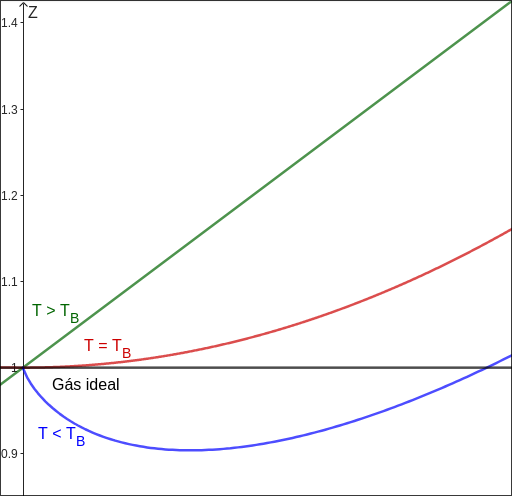
\includegraphics[width=.4\linewidth]{images/geo3b.png}
        \caption{Relação entre Z e P para curvas isotérmicas}
        \label{geo3b.png}
    \end{figure}
\end{rsl}
